\documentclass[article,amsmath,amsfonts,amssymb,letterpaper]{standalone}
\usepackage{graphicx}
\usepackage{grffile}
\usepackage{subfigure}
\usepackage{tikz}
\usepackage{circuitikz}
\usepackage{mathtools}

%\usepackage{textcomp}
%\usepackage[bitstream-charter]{mathdesign}
%
%\usepackage[T1]{fontenc}

\usepackage{pgfplotstable}
\usepackage{pgfplots}

\usetikzlibrary{matrix,decorations.text,decorations.pathmorphing,decorations.markings,arrows,arrows.meta,calc,shapes.geometric,patterns,shadows,intersections,decorations.markings,decorations.pathreplacing,decorations.pathreplacing,backgrounds,math}

\begin{document}
\begin{tikzpicture}

\node[anchor=south west,inner sep=0pt] at (0,0) {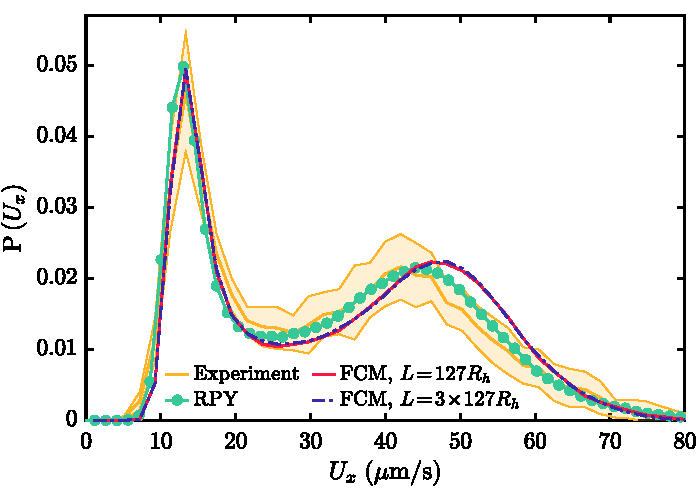
\includegraphics{rollers.pdf}};

% The following parameters need to be set from the m file rollers.m
\newcommand{\x}{1.758958333333334in}; %x0
\newcommand{\y}{1.953893129770993in}; %y0
\newcommand{\Width}{2.8in}; %W

\begin{scope}{background}
  \node[anchor=south west,inner sep=0pt] at (\x,\y) {\resizebox{\Width}{!}{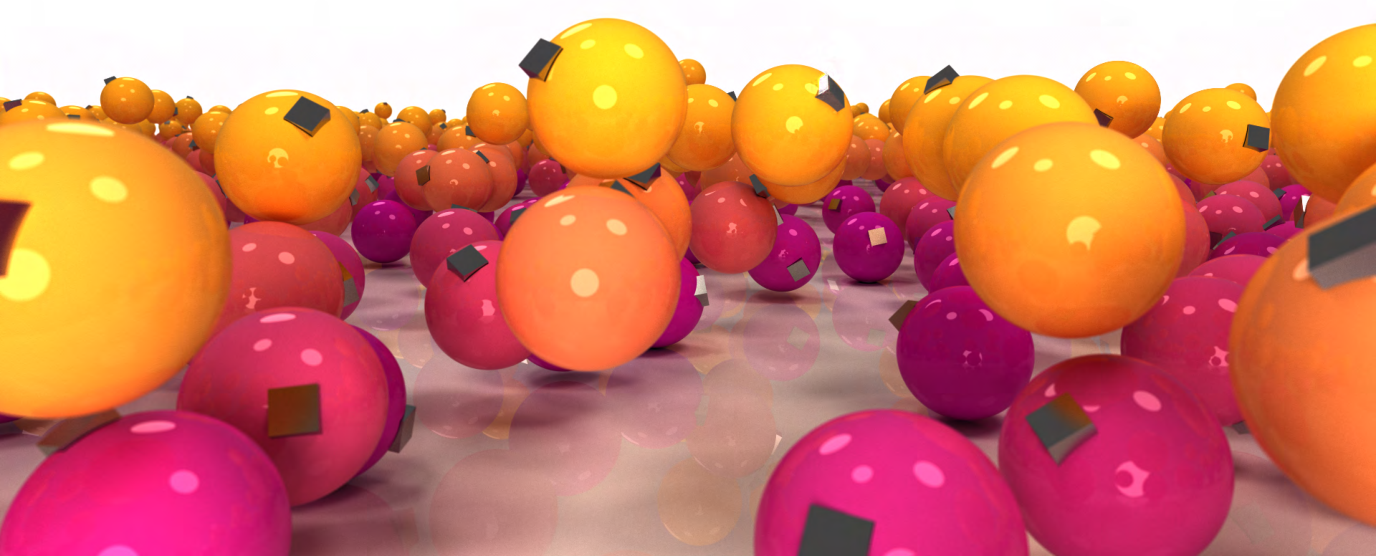
\includegraphics{rollers_inset.pdf}}};
\end{scope}

\end{tikzpicture}

\end{document}
